\documentclass[12pt,oneside]{article}

%%%%%%%%%%%%%%%%%%%%%%%%%%%%
%%   Zusätzliche Pakete  %%
%%%%%%%%%%%%%%%%%%%%%%%%%%%%
\usepackage{enumerate}  
\usepackage{a4wide}
\usepackage{fancyhdr}
\usepackage{graphicx}
\usepackage{tikz}
\usepackage{palatino}
\usepackage{blindtext}
\usepackage{multirow}
\usepackage[ruled,longend]{algorithm2e}
\usepackage{float}
\usepackage[nohyperlinks]{acronym}


% folgende Zeile auskommentieren für englische Arbeiten
\usepackage[ngerman]{babel}

\usepackage[T1]{fontenc}
\usepackage[utf8]{inputenc}
\usepackage[utf8]{inputenc}

%Hervorherbung für Links entfernen
%\usepackage[bookmarks]{hyperref}
\usepackage[bookmarks, pdfborder={0 0 0}]{hyperref}

\usepackage[justification=centering]{caption}
\usepackage{csquotes}

% APA Style für Bibtex
\usepackage[style=apa,natbib=true,backend=biber]{biblatex}

\DefineBibliographyStrings{german}{
  bibliography = {Literaturverzeichnis},
}
\DefineBibliographyStrings{english}{
  bibliography = {References},
}
\bibliography{literatur}

%%%%%%%%%%%%%%%%%%%%%%%%%%%%%%
%% Definition der Kopfzeile %%
%%%%%%%%%%%%%%%%%%%%%%%%%%%%%%

\pagestyle{fancy}
\fancyhf{}
\cfoot{\thepage}
\setlength{\headheight}{16pt}

%%%%%%%%%%%%%%%%%%%%%%%%%%%%%%%%%%%%%%%%%%%%%%%%%%%%%
%%  Definition des Deckblattes und der Titelseite  %%
%%  Do not edit                                    %%
%%%%%%%%%%%%%%%%%%%%%%%%%%%%%%%%%%%%%%%%%%%%%%%%%%%%%

\newcommand{\UDOTitle}[9]{

  \thispagestyle{empty}
  
\includegraphics[width=3in,height=1.09in]{abbildungen/FH_Dortmund-logo.png}
  \vspace*{\stretch{1}}
  \\
  {\parindent0cm
  \rule{\linewidth}{.1ex}}
  \begin{flushright}
    \vspace*{\stretch{1}}
    \sffamily\bfseries\Huge
    #1\\
    \vspace*{\stretch{1}}
    \sffamily\bfseries\large
    #2\\
    \vspace*{\stretch{1}}
  \end{flushright}
  \rule{\linewidth}{.1ex}

  \vspace*{\stretch{1}}
  \begin{center}

    \vspace*{\stretch{1}}
    \large #5\\

    \vspace*{\stretch{1}}
    \large Studiengang: #4 \\[1mm]
    \large Matrikelnummer: #3\\[1mm]
    \large Erstgutachter:  #8 \\[1mm]
    \large Zweitgutachter:  #9 \\[1mm]

    \vspace*{\stretch{1}}
    \large Bearbeitungszeit: #6 -- #7

    \vspace*{\stretch{2}}
    \large Lehrstuhl für Enterprise Computing\\
    \large Fakultät für Informatik\\
  \end{center}
}


%%%%%%%%%%%%%%%%%%%%%%%%%%%%
%%  Beginn des Dokuments  %%
%%%%%%%%%%%%%%%%%%%%%%%%%%%%

\begin{document}
\sloppy

  \UDOTitle
      {Entwicklung eines Multi-Agenten-Systems zur KI-gestützten Code-Migration} % Titel der Arbeit
      {Besel, Igor}                           % Vor- und Nachname des Autors
      {1234567}                                     % Matrikelnummer des Autors
      {Bachelor (Angewandte) Informatik}     % Studiengang
      {Projektarbeit}   % Art der Arbeit
      {dd.mm.yyyy}                                  % Tag der Anmeldung
      {dd.mm.yyyy}                                  % Tag der Abgabe
      {Prof. Dr. Sven Jörges}                % Name des Erstgutachters
      {N.N.}                                        % Name des Zweitgutachters
      
  \clearpage

%%%%%%%%%%%%%%%%%%%%%%%%%%%%
%%  Zusammenfassung   %%
%%%%%%%%%%%%%%%%%%%%%%%%%%%%
\pagenumbering{Roman} 
    \setcounter{page}{1}
    
\markboth{Zusammenfassung}{Zusammenfassung}
\section*{Zusammenfassung}

Die vorliegende Projektarbeit untersucht, wie ein Multi-Agenten-System zur KI-gestützten Code-Migration gestaltet werden kann. Ausgangspunkt ist die Beobachtung, dass Reverse Engineering und Re-Implementierung gewachsener Softwaresysteme in der Praxis häufig an hoher kognitiver Last, fehlender Dokumentation und technologischen Paradigmenwechseln scheitern. Direkte Transpilierungsansätze reichen dabei oft nicht aus, um fachliche und architektonische Intentionen zuverlässig in ein Zielsystem zu überführen.

Als methodischer Rahmen wird daher ein Ansatz verfolgt, der Spec-Driven Reverse Engineering mit einer anschließenden Re-Implementierung verbindet. Bestehender Quellcode soll zunächst analysiert und in textuelle technische Spezifikationen überführt werden, bevor auf dieser Grundlage Zielcode erzeugt wird. Die Spezifikation fungiert dabei als zentrales Zwischenartefakt zwischen Wissensextraktion und Code-Synthese. Zur Umsetzung wird eine orchestrierte Pipeline spezialisierter Agenten konzipiert, die Rollen für Analyse, Spezifikation, Verifikation und Generierung übernehmen.

Technisch stützt sich der Ansatz auf das Model Context Protocol, um Analysewerkzeuge, Code-Repräsentationen und weitere Hilfsdienste standardisiert einzubinden. Ergänzend wird Context Engineering genutzt, um den Wissenszugriff für einzelne Agenten gezielt zu steuern und relevante Informationen bedarfsorientiert bereitzustellen. Dadurch soll der Umgang mit Kontext-Limits großer Sprachmodelle verbessert und das Risiko von Halluzinationen reduziert werden.

Ziel der Arbeit ist ein prototypischer Proof of Concept an einem repräsentativen Quell-Modul. Die Evaluation orientiert sich an den Kriterien Vollständigkeit im Sinne von Feature Parity, Qualität und Wartbarkeit der erzeugten Artefakte sowie an der Nachvollziehbarkeit der Migrationsentscheidungen. Die Arbeit schafft damit eine konzeptionelle Grundlage für eine spätere wissenschaftliche Vertiefung im Rahmen der Bachelorarbeit, insbesondere im Hinblick auf hybride Ansätze aus textuellen Spezifikationen und visuellen Modellen.

\clearpage

%%%%%%%%%%%%%%%%%%%%%%%%%%%%
%%  Abstract   %%
%%%%%%%%%%%%%%%%%%%%%%%%%%%%
% \markboth{Abstract}{Abstract}
% \section*{Abstract (nur bei Bachelor- und Masterthesis)}
% Zusammenfassung in englischer Sprache.

\clearpage

\lhead{}

\tableofcontents
\thispagestyle{empty}
\clearpage

\pagenumbering{Roman} 
    \setcounter{page}{3}

\addcontentsline{toc}{section}{\listfigurename}
\listoffigures
\clearpage

\addcontentsline{toc}{section}{\listtablename}
\listoftables
\clearpage

\addcontentsline{toc}{section}{Abkürzungsverzeichnis}
% !TEX root = main.tex

\section*{Abkürzungsverzeichnis}
% nur bei Bachelor- und Masterthesis

\begin{acronym}[LLM] %Wert in eckiger Klammer ist durch die längste Abkürzung zu substituieren

\acro{LLM}{Large Language Model}
\acro{MCP}{Model Context Protocol}
\acro{MDD}{Model-Driven Development}
\acro{PoC}{Proof of Concept}
\acro{RE}{Reverse Engineering}
\acro{SDD}{Spec-Driven Development}

\end{acronym}

\clearpage

% Formelverzeichnis können an dieser Stelle sinnvolle Ergänzungen sein.

%%%%%%%%%%%%%%%%%%%%%%%%%%%%
%%  Einstellungen  %%
%%%%%%%%%%%%%%%%%%%%%%%%%%%%
\cleardoublepage
\pagenumbering{arabic}  
    \setcounter{page}{1}
\lhead{\nouppercase{\leftmark}}

%%%%%%%%%%%%%%%%%%%%%%%%%%%%
%%  Hauptteil  %%
%%%%%%%%%%%%%%%%%%%%%%%%%%%%

%Kapitel mit Seitenumbruch
\section{Einleitung} \label{einleitung}

Dieses Kapitel führt in die Motivation, den Lösungsansatz, die Zielsetzung und die Abgrenzung der Projektarbeit ein.

\subsection{Herausforderungen von Reverse Engineering und Re-Implementierung}

Das Reverse Engineering und die Re-Implementierung bestehender Codebasen zählen zu den zentralen Herausforderungen der zeitgenössischen Softwareentwicklung. Im Lebenszyklus gewachsener Systeme entstehen technologisch bedingte Grenzen hinsichtlich Performance, Wartbarkeit und Skalierbarkeit, sodass ein Wechsel auf moderne Sprachen und Architekturen erhebliche Vorteile verspricht. Dazu zählen insbesondere verbesserte Typsicherheit, höhere Ressourceneffizienz und nativer Concurrency-Support. Sowohl klassische modellgetriebene Arbeiten als auch aktuelle Übersichten zu LLM-gestütztem Reverse Engineering ordnen diese Transformationsaufgabe als besonders anspruchsvoll ein \parencite{raibulet2017mdre,hu2025sokreverseengineering}.

In der Praxis scheitert eine solche Migration jedoch häufig an der hohen kognitiven Last für Entwickler, einer lückenhaften Dokumentation des Bestands sowie an grundlegenden Paradigmenwechseln zwischen Quell- und Zieltechnologie. Gerade die Überführung bestehender Systeme in explizite, rekonstruierbare Anforderungen bildet daher eine zentrale Brücke zwischen Reverse Engineering und späterer Neuimplementierung \parencite{fahmi2007reverse}.

\subsection{Spec-Driven Development durch Agentenorchestrierung}

Als Lösungsansatz wird eine Migrationsstrategie verfolgt, die nicht auf direkter Transpilierung basiert, sondern auf einer vorgelagerten Spezifikationsebene. Im Sinne von Spec-Driven Development (SDD) wird der bestehende Quellcode zunächst in technische Anforderungen und Verhaltensbeschreibungen überführt, bevor die Implementierung in der Zielsprache erfolgt. Eine solche explizite Spezifikation ist auch deshalb vielversprechend, weil präzise Angaben zu I/O-Formaten, Bedingungen und Beispielen die Zuverlässigkeit nachgelagerter Codegenerierung erhöhen \parencite{midolo2026promptguidelines}.

Die Erstellung, Prüfung und Nutzung dieser Spezifikationen soll durch einen orchestrierten Verbund spezialisierter Agenten erfolgen. Dadurch werden Analyse, Spezifikation, Verifikation und Generierung in klar abgegrenzte Rollen zerlegt. Vergleichbare arbeitsteilige Muster wurden bereits in agentischen Software-Engineering-Ansätzen untersucht \parencite{qian2024chatdev,yang2024sweagent}.

\subsection{Zielsetzung der Migrations-Pipeline}

Ziel der Projektarbeit ist die Konzeption und prototypische Implementierung einer automatisierten Migrations-Pipeline auf Basis eines Multi-Agenten-Systems (MAS). Der Prototyp soll zeigen, dass sich aus bestehendem Quellcode präzise technische Spezifikationen in Markdown gewinnen lassen, die anschließend als belastbare Grundlage für die Code-Generierung dienen. Die technische Kopplung zwischen Agenten und Analysewerkzeugen wird dabei bewusst über standardisierte Schnittstellen gedacht \parencite{mcpdocs}.

Der angestrebte Proof of Concept konzentriert sich auf ein repräsentatives Quell-Modul. Damit soll ein vollständiger Durchstich durch Analyse, Spezifikation, Verifikation und Generierung demonstriert werden, ohne den Rahmen der Projektarbeit zu überschreiten.

\subsection{Abgrenzung auf textbasierte Spezifikationen}

Die Projektarbeit fokussiert auf textbasierte technische Spezifikationen als zentrales Zwischenartefakt. Visuelle Modelle stehen noch nicht im Zentrum des prototypischen Umsetzungsumfangs. Diese Abgrenzung erlaubt es, zunächst die Qualität textueller Anforderungen, ihrer Verifikation und ihrer Wirkung auf die nachgelagerte Codeerzeugung in den Vordergrund zu stellen \parencite{midolo2026promptguidelines,korn2026reportingprompting}.

Nicht Ziel ist die vollständige Automatisierung beliebiger Migrationsszenarien, sondern die nachvollziehbare Demonstration eines Kernprozesses innerhalb eines überschaubaren Anwendungsfalls.

\section{Grundlagen} \label{grundlagen}

Dieses Kapitel ordnet die technischen und methodischen Grundlagen der Arbeit ein.

\subsection{Reverse Engineering, Re-Engineering und Forward Engineering}

Reverse Engineering, Re-Engineering und Forward Engineering bilden den klassischen begrifflichen Rahmen, in dem auch die vorliegende Arbeit verortet ist. Nach der Taxonomie von \textcite{chikofsky1990taxonomy} dient Reverse Engineering dazu, ein bestehendes System zu analysieren, seine Komponenten und Beziehungen zu identifizieren und daraus höherwertige Repräsentationen abzuleiten. Forward Engineering beschreibt dagegen den Weg von solchen Abstraktionen zurück in eine Implementierung. Re-Engineering verbindet beide Richtungen zu einem Erneuerungsprozess, bei dem ein bestehendes System verstanden, restrukturiert und in veränderter technischer Form neu umgesetzt wird \parencite{chikofsky1990taxonomy,raibulet2017mdre}.

Für gewachsene Softwaresysteme ist diese Unterscheidung besonders relevant, weil Migrationen in der Regel nicht als direkte Code-zu-Code-Übersetzung gelingen. Vielmehr muss der Bestandscode zunächst semantisch erschlossen werden, bevor fachliche Logik, Architekturentscheidungen und Randbedingungen in einer neuen technologischen Umgebung wieder implementiert werden können. Klassische Arbeiten zum Reverse Engineering objektorientierter Systeme betonen daher die Notwendigkeit, Codewissen schrittweise auf höhere Abstraktionsebenen zu heben \parencite{tonella2005reverseoo}.

\subsubsection{Horseshoe-Modell als Referenzrahmen}

Ein verbreitetes Denkmuster für diesen Ablauf ist das Horseshoe-Modell des Re-Engineering. Es veranschaulicht, dass der Weg von einem Quellsystem nicht direkt in eine Zielimplementierung führt, sondern über eine abstrahierte Zwischenebene verläuft, auf der Modelle, Architektursichten oder Spezifikationen explizit gemacht werden. Modellgetriebene Reverse-Engineering-Ansätze nutzen genau diese Zwischenebene als Brücke zwischen Analyse und Neuimplementierung \parencite{raibulet2017mdre}.

\begin{figure}[H]
\centering
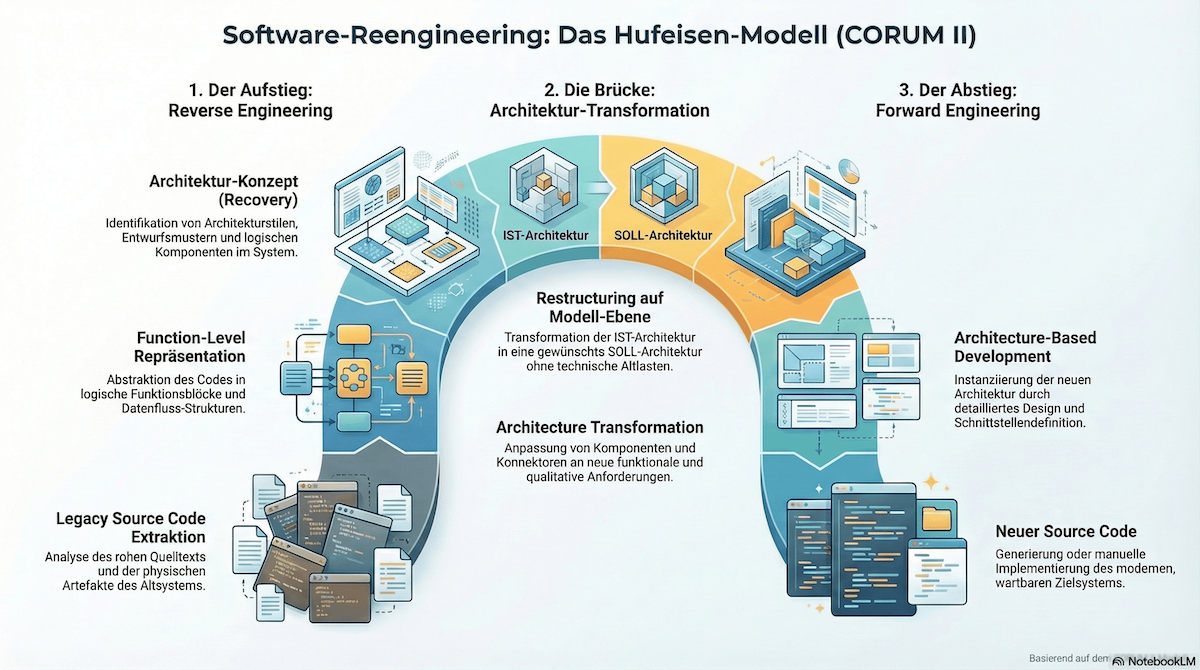
\includegraphics[width=0.9\textwidth,height=0.5025\textwidth,keepaspectratio]{abbildungen/horseshoe-modell.png}
\caption{Schematische Darstellung des Horseshoe-Modells für das Re-Engineering in Anlehnung an \textcite{raibulet2017mdre}.}
\label{fig:horseshoe-model}
\end{figure}

In der vorliegenden Arbeit wird diese Abstraktionsebene nicht primär durch formale Modelle, sondern durch textuelle technische Spezifikationen realisiert. Damit bleibt das Grundmuster des Re-Engineering erhalten, wird jedoch um einen spec-getriebenen und agentisch orchestrierten Verarbeitungsschritt erweitert.

\subsubsection{Agentenbasierte Code-Migration als Sonderfall des Re-Engineering}

Agentenbasierte Code-Migration beschreibt Migrationsprozesse, bei denen spezialisierte Software-Agenten einzelne Aufgaben des Reverse Engineering, der Wissensextraktion, der Spezifikation und der Code-Erzeugung übernehmen. In der vorliegenden Arbeit wird sie damit nicht als eigenständige Disziplin neben dem Re-Engineering verstanden, sondern als ein KI-gestützter Sonderfall dieses übergeordneten Erneuerungsprozesses. Gegenüber monolithischen Ansätzen verspricht diese Form der Aufgabenteilung eine bessere Nachvollziehbarkeit und klarere Verantwortlichkeiten. Einen aktuellen Überblick über Ansätze mit großen Sprachmodellen im Reverse Engineering geben \textcite{hu2025sokreverseengineering}. Erste Arbeiten behandeln dabei unter anderem generative KI für Re-Engineering-Szenarien in Software-Produktlinien, LLM-gestützte Werkzeugunterstützung im model-driven Reverse Engineering sowie die Ableitung von Sequenzdiagrammen aus Quellartefakten \parencite{acher2023splreengineering,boronat2025mdrellm,greiner2025sequencediagrams}.

Ein wesentlicher Schwierigkeitsfaktor der Migration liegt in technologischen Brüchen zwischen Quell- und Zielsystem. Unterschiede in Typisierung, Laufzeitmodell, Fehlerbehandlung oder Nebenläufigkeit erschweren eine rein syntaktische Übertragung und machen eine semantische Rekonstruktion der Fachlogik erforderlich. Werden große Sprachmodelle (Large Language Models, LLMs) in solchen Migrationsprozessen eingesetzt, entsteht zusätzlich die Herausforderung nicht-deterministischer Ausgaben. Halluzinationen und inkonsistente Ableitungen gefährden insbesondere bei umfangreichen Codebasen die Korrektheit der Ergebnisse. Deshalb müssen generierte Artefakte gegen belastbare Quellinformationen überprüft werden.

\subsection{Spec-Driven Development}

Spec-Driven Development verlagert den Schwerpunkt der Migration von der unmittelbaren Code-Erzeugung auf eine vorgelagerte Beschreibung der fachlichen und technischen Anforderungen. Die Spezifikation fungiert dabei als Zwischenartefakt, das sowohl der Analyse als auch der späteren Generierung als Referenz dient. Auf der Ebene aktueller KI-Werkzeuge beschreibt \textcite{boeckeler2025sdd} diesen Ansatz als Verschiebung von einem reinen ``Prompt-to-Code''-Muster hin zu einem Vorgehen, bei dem zunächst ein belastbares Spec-Artefakt erzeugt und anschließend als Anker für weitere Implementierungsschritte genutzt wird.

\begin{figure}[H]
\centering
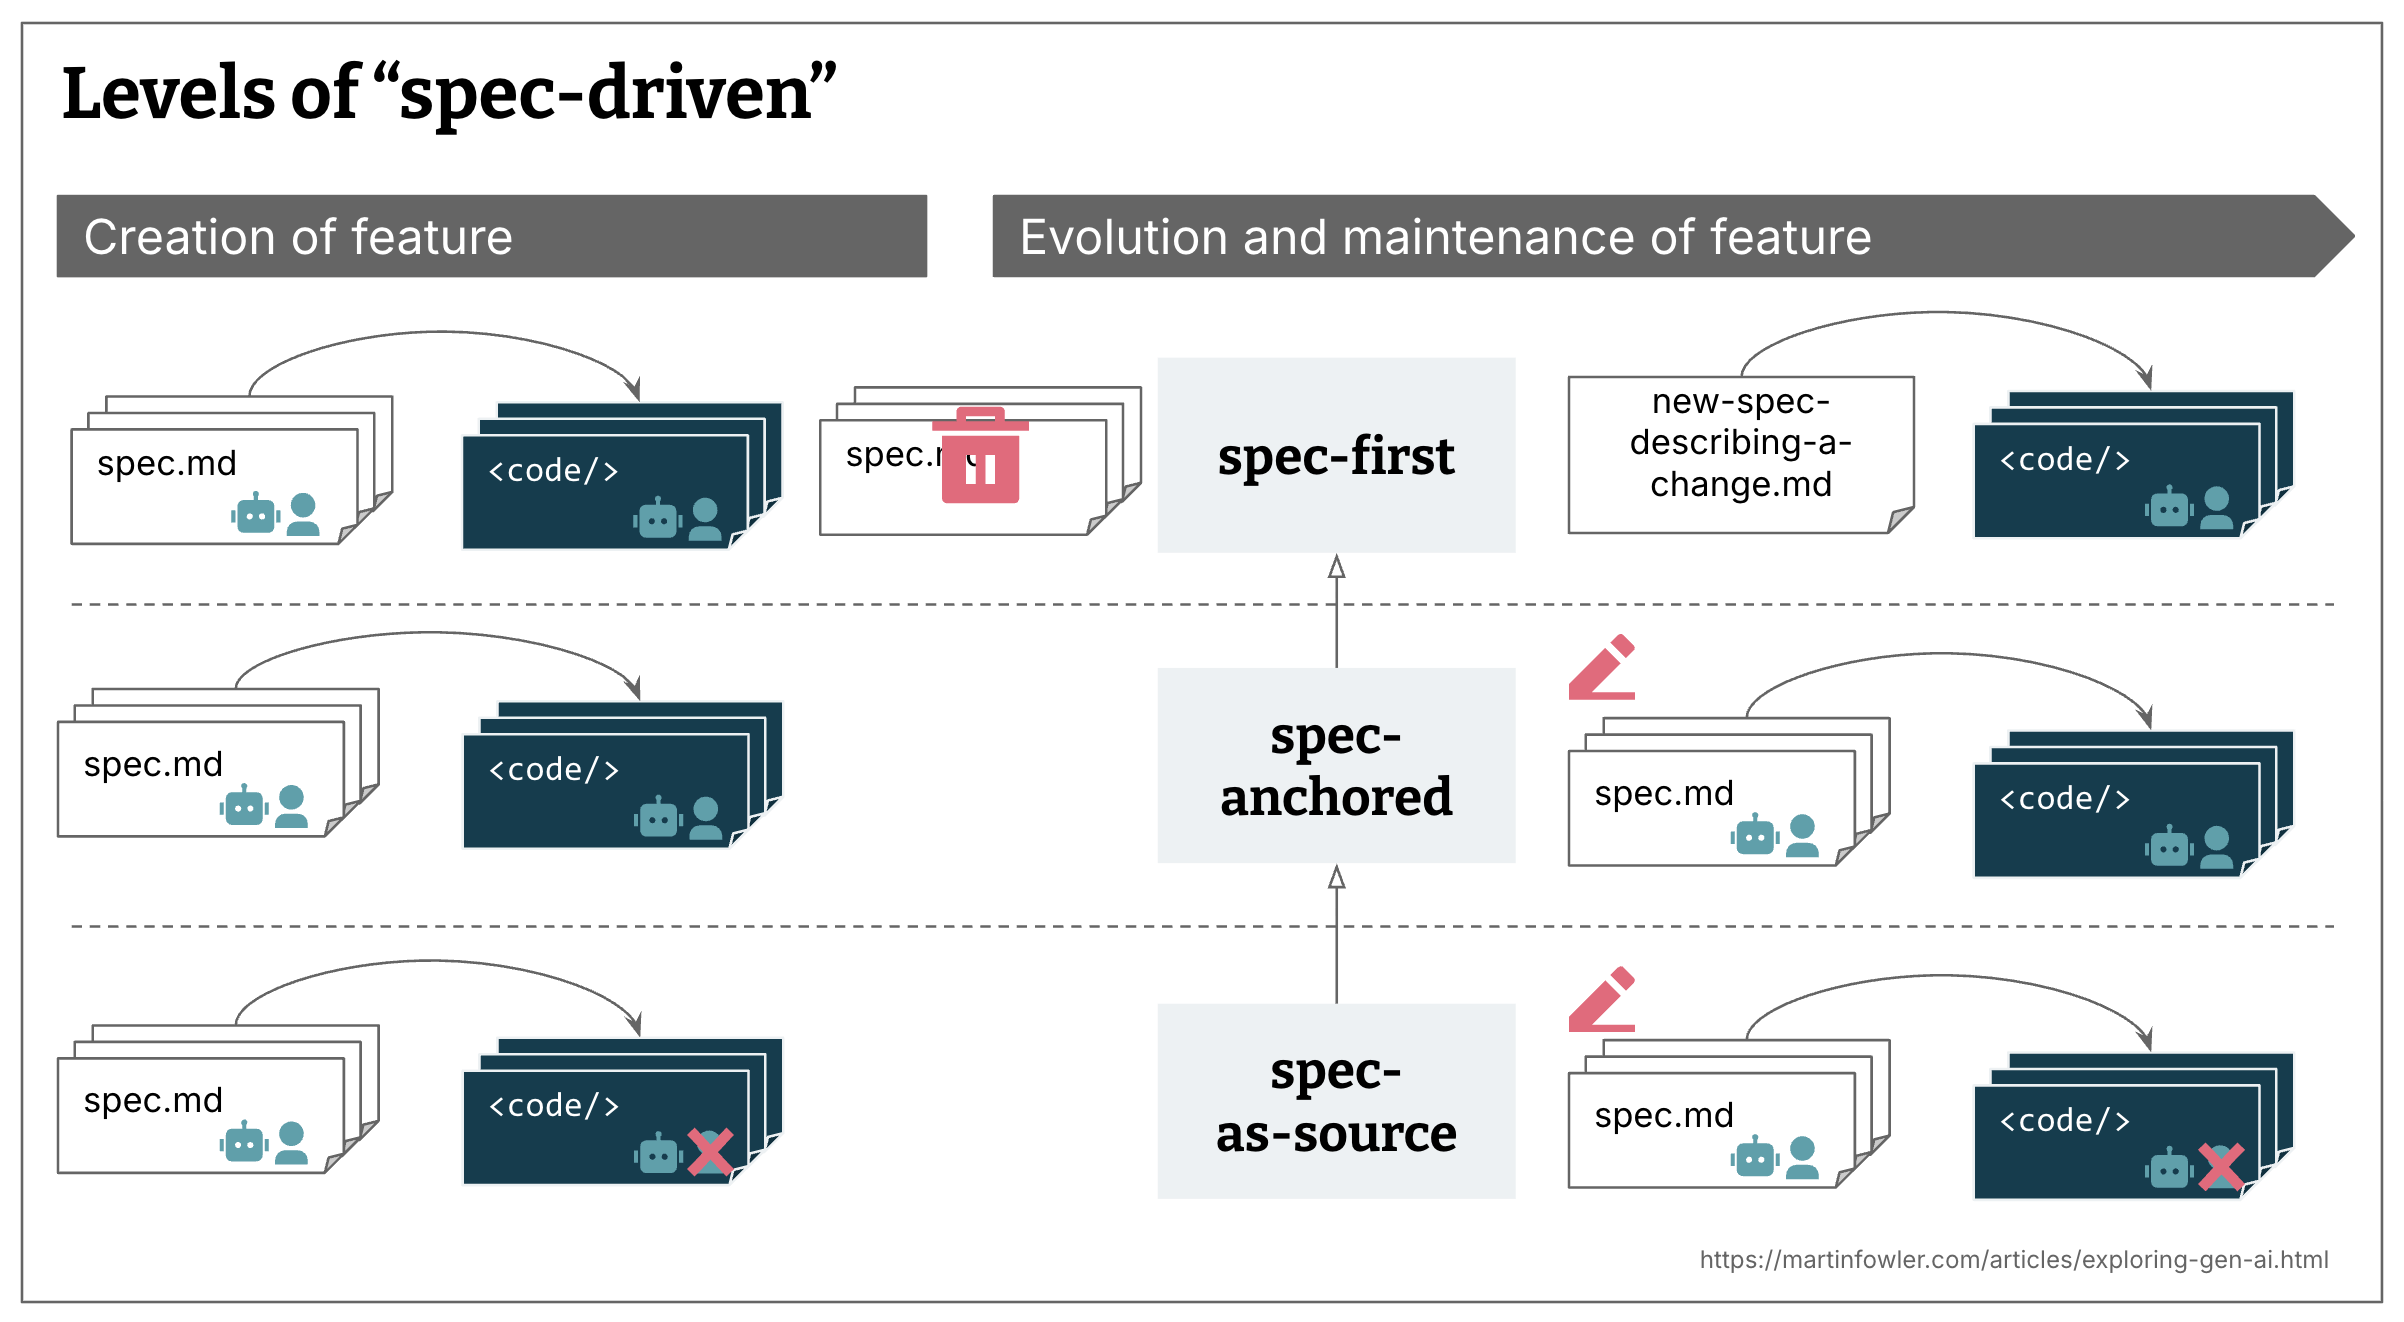
\includegraphics[width=0.9\textwidth,height=0.4948\textwidth,keepaspectratio]{abbildungen/fowler-sdd-levels.png}
\caption{Abbildung zu Ausprägungen und Reifegraden von Spec-Driven Development aus \textcite{boeckeler2025sdd}. Für die vorliegende Projektarbeit ist insbesondere die spec-first Ausprägung relevant, in der zunächst ein belastbares Spezifikationsartefakt erzeugt wird, bevor die eigentliche Implementierung beginnt.}
\label{fig:sdd-varianten}
\end{figure}

\subsubsection{Das Konzept „Specification First“ im Software-Reengineering}

Im Software-Reengineering bedeutet ``Specification First'', dass vorhandene Systemlogik zunächst rekonstruiert und in eine explizite technische Beschreibung überführt wird. Dadurch wird Wissen aus schwer zugänglichem Bestandscode in eine Form gebracht, die überprüfbar und transformierbar ist. Für die Überführung des vorhandenen Codes in Anforderungen ist dabei die Brücke zwischen Reverse Engineering und Requirements Engineering zentral \parencite{fahmi2007reverse}. Gleichzeitig lässt sich dieser Gedanke mit Fowlers Verständnis von Spezifikationen als präzisierenden Arbeitsartefakten verbinden: In ``Specification by Example'' argumentiert \textcite{fowler2004specificationbyexample}, dass Beispiele und konkretisierte Verhaltensbeschreibungen nicht bloß Dokumentation sind, sondern ein Mittel, um Anforderungen, erwartetes Verhalten und spätere Verifikation enger miteinander zu koppeln. Für die vorliegende Arbeit ist dieser Gedanke besonders relevant, weil die technische Spezifikation nicht nur beschreibend, sondern auch prüfbar und für nachgelagerte Agenten operationalisierbar sein soll.

\subsubsection{Vorteile der Abstraktion gegenüber direkter Code-Transpilierung}

Die Abstraktion über Spezifikationen bietet Vorteile gegenüber direkter Transpilierung, weil sie architektonische Intentionen, Fachlogik und Randbedingungen explizit macht. Damit sinkt das Risiko, dass ein Zielsystem zwar syntaktisch korrekt, aber konzeptionell fehlerhaft oder schwer wartbar entsteht. Aus Fowler-Perspektive lässt sich dies zusätzlich über die Idee domänenspezifischer Sprachen und semantischer Modelle begründen: Werden Anforderungen in eine fachlich lesbare, strukturierte Form überführt, entsteht ein robusteres Bindeglied zwischen Problemraum und technischer Umsetzung \parencite{fowler2010dsl}. Für den PoC der Projektarbeit wird keine vollwertige DSL entwickelt, wohl aber ein textuelles Spec-Artefakt mit ähnlicher Funktion: Es strukturiert Fachlogik, Schnittstellen und Randfälle so, dass spätere Generierungsschritte nicht ausschließlich auf impliziten Annahmen im Quellcode oder im Prompt beruhen.

Die empirische Untersuchung von \textcite{midolo2026promptguidelines} legt zudem nahe, dass explizite Angaben zu Ein- und Ausgabeformaten, Vor- und Nachbedingungen sowie Beispielen die Erfolgswahrscheinlichkeit in der nachgelagerten Codegenerierung deutlich erhöhen. Diese Beobachtung stützt den spec-getriebenen Fokus der vorliegenden Arbeit. Im Sinne von \textcite{boeckeler2025sdd} ist die Spezifikation damit nicht nur Dokumentation, sondern das zentrale Koordinationsartefakt zwischen Analyse, Verifikation und Generierung.

Im Kontext des Horseshoe-Modells passt für die vorliegende Projektarbeit vor allem eine spec-first Ausprägung. Zunächst wird die bestehende Funktionalität durch Analyse und Reverse Engineering in ein eigenständiges Spezifikationsartefakt überführt. Erst auf dieser Grundlage beginnt die eigentliche Entwicklung des Zielsystems. Die Spezifikation ist damit nicht nur begleitender Anker, sondern die verbindliche Übergabeschicht zwischen Rekonstruktion und Neuimplementierung. Gerade für einen PoC ist diese Reihenfolge sinnvoll, weil sie den Nutzen expliziter Spezifikation sichtbar macht, ohne bereits einen vollständig modell- oder DSL-basierten Generierungsansatz vorauszusetzen.

\subsection{Multi-Agenten-Systeme und Wissensrepräsentation}

Multi-Agenten-Systeme (MAS) ermöglichen die Zerlegung komplexer Migrationsaufgaben in klar spezialisierte Rollen. Entscheidend ist dabei, dass die beteiligten Agenten nicht nur generieren, sondern auf strukturierte Repräsentationen des Quellkontexts zugreifen können. Die theoretische Basis dafür liefert die Multi-Agenten-Forschung seit Langem \parencite{wooldridge2009multiagent}.

\subsubsection{Rollendekomposition in Analyse, Spezifikation und Verifikation}

Die Rollendekomposition in Analyse, Spezifikation, Verifikation und Implementierung schafft eine nachvollziehbare Prozessstruktur. Jeder Agent bearbeitet nur einen begrenzten Aufgabenbereich, wodurch Ergebnisse gezielter geprüft werden können.

\subsubsection{Der Code Knowledge Graph als deterministisches Kontext-Gedächtnis}

Ein Code Knowledge Graph dient als strukturierte Repräsentation von Symbolen, Abhängigkeiten und Beziehungen innerhalb der Codebasis. Als deterministisches Kontext-Gedächtnis kann er Agenten gezielt mit belastbaren Informationen versorgen und damit die Abhängigkeit von unstrukturiertem Prompt-Kontext verringern. Für den Proof of Concept wird diese Funktion konkret über Sourcebot gedacht, das als Code-Intelligence-Schicht sowie als MCP-anbindbares Werkzeug einen praktischen Zugriff auf Repository-Strukturen, Symbole, Referenzen und dateibasierte Codekontexte ermöglicht \parencite{sourcebotdocs}.

\subsection{Model Context Protocol als Integrationsstandard}

Das Model Context Protocol (MCP) bildet in der vorliegenden Arbeit den Integrationsstandard zwischen Agenten und externen Werkzeugen. Es ermöglicht, Analysefunktionen, Datenquellen und Hilfsdienste standardisiert bereitzustellen \parencite{mcpdocs}. Im geplanten Werkzeugzuschnitt übernimmt Sourcebot dabei die Rolle der Code-Intelligence für Repository-Strukturen, Symbolauflösung und Referenzsuche, während Context7 als ergänzender MCP-Zugriff für bibliotheks- und dokumentationsbezogenen Referenzkontext vorgesehen ist \parencite{sourcebotdocs,context7docs}.

\subsubsection{Architektur, Ressourcen, Prompts und Werkzeuge}

MCP unterscheidet funktional zwischen Resources, Prompts und Tools. Dadurch können sowohl statische Informationen als auch aktive Analyseoperationen kontrolliert in agentische Workflows eingebunden werden.

\subsubsection{Kontext-Management durch Entkopplung von Agenten und Werkzeugen}

Die Entkopplung von Agenten und Tooling erleichtert ein effizientes Kontext-Management. Statt große Quelltextmengen dauerhaft im Kontextfenster eines Modells zu halten, können Informationen bedarfsorientiert abgefragt werden. Dies ist eine zentrale Voraussetzung für die Analyse umfangreicher Codebasen innerhalb begrenzter Token-Limits. Im geplanten PoC übernimmt Sourcebot dabei die Rolle einer MCP-gebundenen Code-Intelligence und unterstützt so insbesondere den Analyzer beziehungsweise Modeler bei der kontextarmen, aber zielgerichteten Erschließung des Bestands.

\subsection{Context Engineering und Wissenszugriff}

Context Engineering beschreibt in der vorliegenden Arbeit die gezielte Auswahl, Aufbereitung und Bereitstellung von Kontext für einzelne Agentenrollen. Ziel ist es, jedem Arbeitsschritt genau die Informationen bereitzustellen, die für Analyse, Spezifikation, Verifikation oder Generierung benötigt werden. Diese Einordnung wird durch aktuelle Benchmarking-Arbeiten gestützt, die viele Software-Engineering-Benchmarks als zu arm an Repository-, Prozess- und Dokumentationskontext kritisieren \parencite{rodriguezcardenas2026behelm}.

\subsubsection{Bedarfsorientierte Kontextbereitstellung}

Die bedarfsorientierte Kontextbereitstellung reduziert unnötige Informationslast und unterstützt die Spezialisierung einzelner Agenten. Statt vollständige Codebasen in Prompts zu überführen, werden nur relevante Ausschnitte, Strukturen und Analyseergebnisse zugänglich gemacht.

\subsubsection{Reduktion von Kontextlast durch gezielte Abrufstrategien}

Gezielte Abrufstrategien dienen dazu, die verfügbare Kontextgröße effizient zu nutzen. Dadurch wird das Risiko reduziert, dass wesentliche Informationen im überladenen Kontext untergehen oder Modellantworten durch irrelevante Inhalte verwässert werden.

\subsubsection{Spezifikationen als kuratierte Kontextpakete}

Für die vorliegende Arbeit ist Context Engineering nicht nur eine Frage des Tool-Zugriffs, sondern auch der Form, in der Wissen zwischen Agenten weitergegeben wird. Technische Spezifikationen übernehmen dabei die Rolle kuratierter Kontextpakete: Sie verdichten Analyseergebnisse, Annahmen, Schnittstellen, Randfälle und Akzeptanzkriterien in einer Form, die für nachgelagerte Rollen gezielt nutzbar ist. Praxisnahe Leitfäden zu agentischen Spezifikationen betonen entsprechend, dass Spezifikationen klar strukturiert, rollenübergreifend anschlussfähig und auf konkrete Umsetzungsentscheidungen ausgerichtet sein sollten \parencite{agentskillsspecification}.

Gerade im Zusammenspiel mit MCP wird dieser Gedanke relevant. Während MCP den standardisierten Zugriff auf Werkzeuge, Ressourcen und Prompts ermöglicht, liefert das Spezifikationsartefakt den inhaltlich vorstrukturierten Kontext für die eigentliche Arbeitsphase eines Agenten. Context Engineering bedeutet im PoC damit, nicht den gesamten Bestandscode in einen Prompt zu verlagern, sondern die jeweils benötigte Sicht gezielt aus Quellkontext, MCP-gestützten Abrufen und einem belastbaren Spec-Artefakt zusammenzusetzen. Praktisch kann dies etwa eine Kombination aus Sourcebot als Code-Intelligence für Repository-Wissen und Context7 für externe Framework- und Bibliotheksdokumentation umfassen.

\section{Konzeption der Migrations-Pipeline} \label{konzeption}

Dieses Kapitel beschreibt das konzeptionelle Design der orchestrierten Migrations-Pipeline.

\subsection{Rollen im orchestrierten Workflow}

Der Workflow wird in spezialisierte Rollen zerlegt, um nicht-deterministische Modellantworten durch klare Zuständigkeiten und Zwischenschritte zu kontrollieren. Dadurch entsteht eine Pipeline, in der Ergebnisse schrittweise weiterverarbeitet und überprüft werden. Vergleichbare agentische Rollenkonzepte wurden etwa in ChatDev für Softwareentwicklungsprozesse untersucht \parencite{qian2024chatdev}.

\subsubsection{Analyzer}

Der Analyzer erschließt die bestehende Codebasis mithilfe statischer Analyse und strukturierter Code-Intelligence. Ziel ist die Gewinnung fachlicher und technischer Informationen auf Basis von Symbol- und Abhängigkeitsbeziehungen.

\subsubsection{Spec-Writer}

Der Spec-Writer überführt die Analyseergebnisse in textuelle Spezifikationen. Diese Markdown-Artefakte sollen sowohl für menschliche Prüfung als auch für nachgelagerte Generierungsschritte nutzbar sein.

\subsubsection{Verifier}

Der Verifier prüft, ob die Spezifikation mit dem rekonstruierbaren Quellkontext übereinstimmt. Dadurch wird verhindert, dass implizite Annahmen oder halluzinierte Details unbemerkt in die Implementierung einfließen.

\subsubsection{Builder}

Der Builder erzeugt aus der validierten Spezifikation den Zielcode. Die Erzeugung basiert damit nicht direkt auf dem Ausgangscode, sondern auf einem geprüften Zwischenartefakt.

\subsection{Feedback und iterative Validierung}

Die Pipeline ist als iterativer Prozess mit Rückkopplungsschleifen zu verstehen. Analyseergebnisse, Spezifikationen und Verifikationsergebnisse beeinflussen sich wechselseitig, sodass unklare oder fehlerhafte Ableitungen frühzeitig korrigiert werden können.

\subsubsection{Feedback-Schleifen zwischen Spezifikation und Quell-Kontext}

Feedback-Schleifen zwischen Spezifikation und Quell-Kontext ermöglichen eine schrittweise Schärfung der Anforderungen. Erkennt der Verifier Unstimmigkeiten, müssen Analyzer und Spec-Writer ihre Artefakte gezielt nacharbeiten, bevor eine Implementierung zulässig ist.

\subsubsection{Abgleich mit dem Code Knowledge Graph}

Der automatische Abgleich gegen den Code Knowledge Graph liefert dafür eine deterministische Referenz. Er ermöglicht den Vergleich modellgenerierter Aussagen mit Symbolen, Abhängigkeiten und Strukturen der Ausgangsbasis.

\subsection{Phasenmodell der Pipeline}

Das Phasenmodell der Pipeline gliedert sich in Ingestion, Spec-Generation und Code-Synthese. In der Ingestion wird die Codebasis strukturiert erschlossen, in der Spec-Generation in ein überprüfbares Zwischenartefakt überführt und in der Code-Synthese in eine Zielimplementierung transformiert.

\section{Prototypische Implementierung} \label{implementierung}

Dieses Kapitel beschreibt die prototypische Umsetzung der konzipierten Pipeline.

\subsection{Architektur des Agenten-Workflows (Orchestrierungsebene)}

Die inhaltliche Ausarbeitung dieses Abschnitts folgt in der finalen Fassung.

\subsection{MCP-Integration: Anbindung der statischen Analyse-Engine}

Die inhaltliche Ausarbeitung dieses Abschnitts folgt in der finalen Fassung.

\subsection{Strategien zum Context-Scaling: Gezielter Wissensabruf zur Einhaltung von Token-Limits}

Die inhaltliche Ausarbeitung dieses Abschnitts folgt in der finalen Fassung.

\subsection{Herausforderungen bei der Workflow-Steuerung}

Die inhaltliche Ausarbeitung dieses Abschnitts folgt in der finalen Fassung.

\subsubsection{Mapping von Bibliotheks-Abhängigkeiten}

Die inhaltliche Ausarbeitung dieses Abschnitts folgt in der finalen Fassung.

\subsubsection{Laufzeit-Monitoring und Fehlerbehandlung in Agenten-Dialogen}

Die inhaltliche Ausarbeitung dieses Abschnitts folgt in der finalen Fassung.

\section{Evaluation am Fallbeispiel} \label{evaluation}

Dieses Kapitel demonstriert die Pipeline am konkreten Migrationsszenario und beschreibt, wie die Vollständigkeit der erzeugten Artefakte sichergestellt wird.

\subsection{Auswahl des Szenarios und Quell-Moduls}

Als Demonstrationsszenario dient die Migration eines Node.js-basierten Lizenz-Checkers nach Go. Das Modul wurde gewählt, weil es ausreichend fachliche und technische Komplexität besitzt, um einen vollständigen Durchstich durch alle Pipelinephasen zu zeigen, ohne den Rahmen der Projektarbeit zu überschreiten. Es umfasst eine Kommandozeilenschnittstelle, Datei- und Verzeichnisverarbeitung, die Auswertung von Paketmetadaten sowie die Ausgabe strukturierter Lizenzberichte. Diese Funktionalitäten lassen sich klar in einzelne Use Cases zergliedern, sodass die Spec-Writer-Fan-out-Logik des Orchestrators gezielt demonstriert werden kann. Das Modul enthält externe Abhängigkeiten, die ein konkretes Bibliotheks-Mapping zwischen Node.js- und Go-Ökosystem erfordern, und besitzt hinreichend definiertes Ein- und Ausgabeverhalten für einen manuellen Input-Output-Vergleich im Evaluationsschritt.

\subsection{Durchführung des spezifikationsgetriebenen Workflows}

Dieser Abschnitt dokumentiert den Ausführungsstand der Pipeline. Die drei Phasen wurden vollständig durchlaufen und alle Artefakte erzeugt. Der abschließende Black-Box-Vergleich zwischen Quell- und Zielsystem wurde manuell nach dem in Abschnitt~\ref{sec:funktionale-validierung} beschriebenen Verfahren durchgeführt; die Befunde sind in Abschnitt~\ref{sec:io-befunde} dokumentiert. Im Zuge des Vergleichs traten zwei methodisch eigenständige Defektklassen zutage, die in iterativen Skill-Anpassungen aufgearbeitet wurden (Abschnitte~\ref{sec:builder-gap} und~\ref{sec:datafluss-gap}).

Im Fallbeispiel wurde die vollständige Pipeline ausgeführt. Der Orchestrator steuerte die Übergaben zwischen den sechs fachlichen Subagenten (Analyzer, Spec-Writer, Architect, Planner, Task Decomposer, Builder) sowie dem Verifier als unabhängiger Prüfinstanz, sodass Analyse, Spezifikation, Architektur, Planung, Aufgabenzerlegung und Code-Synthese vollständig durchgeführt wurden. Der abschließende I/O-Vergleich gegen das Quellsystem wurde anschließend manuell durchgeführt; die Befunde sind in Abschnitt~\ref{sec:io-befunde} dokumentiert.

In Phase~1 erschließt der Analyzer die Quellbasis und erzeugt \texttt{ANALYSIS.md} und \texttt{FUNCTIONALITY-INDEX.md}. Die ausgeführte Pipeline identifizierte acht Funktionalitätselemente: F-001 (CLI-Optionsmodell und Normalisierung), F-002 (Abhängigkeitsgraph-Laden und Traversierungssteuerung), F-003 (Abflachen des Graphen zu einem Modulinventar), F-004 (Lizenzerkennungs- und Normalisierungspipeline), F-005 (Filterung, Paketeinschränkung und Policy-Exits), F-006 (Ausgabe-Rendering und Persistenz), F-007 (Custom-Format und JSON-Konfigurationsladung) sowie F-008 (Stack-Utility-Lifecycle). Alle acht wurden vom Analyzer als \emph{ready} klassifiziert. Der Orchestrator löste daraufhin acht parallele Spec-Writer-Läufe aus, einer pro Funktionalitätselement, und sammelte die Ergebnisse in \texttt{SPEC-INDEX.md}.

In Phase~2 leitete der Architect aus der konsolidierten Spezifikationsbasis eine Go-Zielarchitektur ab: Paketstruktur, Fehlerbehandlungskonventionen, geeignete Standardbibliotheksfunktionen und externe Go-Bibliotheken wurden mit Context7-Unterstützung festgelegt. Der Planner überführte diese Entscheidungen anschließend in einen geordneten Migrationsplan. In Phase~3 zerlegte der Task Decomposer den Plan in umsetzbare Arbeitseinheiten und der Builder erzeugte Go-Zielcode, der in \texttt{BUILD.md} mit Verifikationsnachweis dokumentiert ist. Alle acht Funktionalitäten wurden vollständig durch die Pipeline geführt; der abschließende Vergleich des beobachtbaren CLI-Verhaltens zwischen Quell- und Zielsystem erfolgte anschließend manuell nach dem in Abschnitt~\ref{sec:funktionale-validierung} beschriebenen Verifikationsplan; die Befunde sind in Abschnitt~\ref{sec:io-befunde} dokumentiert.

\subsection{Beispiel: Spezifikation und Zielcode im Vergleich}

Die folgenden Listings zeigen den tatsächlichen Output der Pipeline für die Funktionalität \textbf{F-004: License detection and normalization pipeline}. Listing~\ref{lst:spec} gibt einen Auszug aus der vom Spec-Writer erzeugten \texttt{SPEC.md}, Listing~\ref{lst:target} den daraus vom Builder generierten Go-Zielcode.

\begin{lstlisting}[style=codestyle, caption={Auszug aus der erzeugten SPEC.md fuer F-004 (License detection and normalization pipeline)}, label=lst:spec]
## Requirements

- FR-001: System MUST resolve license from metadata fields
          (`license`, `licenses`) before fallback mechanisms.
- FR-002: System MUST apply fallback precedence:
          metadata -> README-derived -> license-file-derived.
- FR-004: System MUST mark heuristically inferred values
          with trailing `*` to distinguish inferred vs direct.
- FR-005: System MUST normalize URL/file-style references
          to `Custom: <value>`.
- FR-006: File fallback MUST follow deterministic order:
          LICENSE*, LICENCE*, COPYING, README.

## Acceptance Scenario (P1)

Given a module with a valid SPDX `license` string,
When the pipeline resolves license data,
Then that SPDX value is returned without file-based fallback.

## Open Decisions

- OD-001: When `license` and `licenses` conflict, confirm
  exact legacy tie-break order from source code/tests.
- OD-002: Confirm exact fallback value when no license
  signal is found across metadata, README, and files.
\end{lstlisting}

\begin{lstlisting}[style=codestyle, language=Go, caption={Vom Builder erzeugter Go-Zielcode: license/detect.go}, label=lst:target]
package license

import "theseus/target/internal/core"

type Detector struct{}

func (Detector) Resolve(
    input core.ModuleLicenseInput,
) (core.NormalizedLicenseValue, string) {

    // FR-001/FR-002: metadata first
    if v := resolveFromMetadata(input); v != "" {
        return core.NormalizedLicenseValue(v), ""
    }
    // FR-002: README fallback
    if v, _ := normalize(input.ReadmeText); v != "" {
        return core.NormalizedLicenseValue(v), "README"
    }
    // FR-002/FR-006: deterministic file fallback
    for _, candidate := range orderedCandidates(
        input.CandidateFiles,
    ) {
        if v, _ := normalize(candidate.Content); v != "" {
            return core.NormalizedLicenseValue(v),
                   candidate.Name
        }
    }
    // OD-002: sentinel until legacy parity confirmed
    return core.NormalizedLicenseValue("UNKNOWN"), ""
}
\end{lstlisting}

Die Listings zeigen den tatsächlichen Output der ausgeführten Pipeline. Die Anforderungen FR-001 bis FR-006 aus \texttt{SPEC.md} sind direkt auf Implementierungsschritte im Go-Zielcode abbildbar: Die Fallback-Reihenfolge (Metadata $\to$ README $\to$ Dateien) entspricht den in der Spezifikation nummerierten Teilschritten, und die beiden offenen Entscheidungen OD-001 und OD-002 sind als Kommentare im generierten Code explizit markiert. Das zeigt, wie der spec-getriebene Ansatz Unsicherheiten aus der Analyse nicht wegabstrahiert, sondern als \emph{NEEDS CLARIFICATION}-Marker durch die gesamte Pipeline trägt, bis sie manuell oder durch weitere Analyse aufgelöst werden können.

\subsection{Funktionale Validierung und Feature Parity} \label{sec:funktionale-validierung}

Die funktionale Validierung folgt einem Black-Box-Ansatz im Sinne des klassischen \emph{Differential Testing}, bei dem zwei Implementierungen desselben Programms mit identischen Eingaben ausgeführt und ihre Ausgaben verglichen werden, ohne dass Annahmen über die interne Struktur erforderlich sind \parencite{mckeeman1998differentialtesting}. Für die LLM-gestützte Code-Übersetzung hat dieses Vorgehen unter dem Begriff der I/O-Äquivalenz aktuelle Aufmerksamkeit erfahren \parencite{eniser2025realworld}. In der vorliegenden Arbeit werden Quell- und Zielimplementierung als geschlossene CLI-Werkzeuge betrachtet und an identischen Eingaben gegeneinander ausgeführt; die Beurteilung der Feature Parity ergibt sich aus dem Vergleich der beobachtbaren Ausgaben. Als Quellsystem dient \texttt{davglass/license-checker}, dessen sechs Use Cases von der Auflistung aller Dependency-Lizenzen über die Erzeugung maschinenlesbarer Compliance-Artefakte bis hin zur Policy-Durchsetzung in CI-Umgebungen reichen und in den Spezifikationen vollständig abgebildet sind. Statische Analysen und Tests des Zielsystems (\texttt{go build}, \texttt{go vet}, \texttt{go test}) dienen lediglich als Vorab-Filter, der sicherstellt, dass das Zielbinär ausführbar und gegen die Akzeptanzszenarien der Spezifikationen abgesichert ist; die Aussage über die Verhaltensgleichheit gegenüber dem Quellsystem entsteht erst durch den nachgelagerten manuellen I/O-Vergleich. Durchführung und Befunde sind in Abschnitt~\ref{sec:io-befunde} dokumentiert.

\subsubsection{Verifikationsverfahren pro Funktionalität}

Damit Abweichungen sich nicht in einem Gesamtoutput verschleiern, wird der Vergleich getrennt nach den acht identifizierten Funktionalitäten geführt. Wo das Zielsystem während Phase~3 bereits Integrationstests mit Golden-Files erzeugt hat (etwa \texttt{render\_export} oder \texttt{license\_resolution\_compat}), werden diese Fixtures wiederverwendet und gegen die Outputs des Quellsystems gespiegelt, statt die Vergleichsmenge neu aufzubauen. Tabelle~\ref{tab:io-vergleich} fasst das Verifikationsverfahren und die konkreten Testszenarien pro Funktionalität zusammen.

\begin{small}
\begin{longtable}{|p{0.7cm}|p{4.0cm}|p{10.5cm}|}
\caption{Black-Box-Verifikationsverfahren je Funktionalität für den I/O-Vergleich zwischen \texttt{davglass/license-checker} (Node.js) und der Go-Zielimplementierung. Wo vorhandene Integrationstests und Golden-Files des Zielsystems verwendbar sind, werden sie als Vergleichsbasis wiederverwendet.} \label{tab:io-vergleich} \\
\hline
\textbf{F} & \textbf{Funktionalität} & \textbf{Black-Box-Verifikationsverfahren} \\
\hline
\endfirsthead

\multicolumn{3}{l}{\textit{Fortsetzung von Tabelle~\ref{tab:io-vergleich}}} \\
\hline
\textbf{F} & \textbf{Funktionalität} & \textbf{Black-Box-Verifikationsverfahren} \\
\hline
\endhead

\hline
\multicolumn{3}{r}{\textit{Fortsetzung auf der nächsten Seite}} \\
\endfoot

\hline
\endlastfoot

001 & CLI-Optionsmodell & Vergleich von Stdout, Stderr und Exit-Code für alle dokumentierten Flag-Kombinationen, für \texttt{-{}-help}/\texttt{-{}-version} sowie für gezielt ungültige Flag-Kombinationen. \\
\hline
002 & Abhängigkeitsgraph laden & Drei Referenz-Repositories durchlaufen: ein flaches Projekt mit wenigen Direkt-Abhängigkeiten, ein mittelgroßes Projekt mit Dev-/Peer-Abhängigkeiten und ein Projekt mit zyklischen Verweisen. Vergleich der traversierten Modulmengen. \\
\hline
003 & Graph abflachen & Vergleich des sortierten Modulinventars über den bereits vorhandenen \texttt{flatten\_contract}-Integrationstest des Zielsystems. Deduplizierung und Zirkel-Guard werden zusätzlich über konstruierte Sonderfälle geprüft. \\
\hline
004 & Lizenzerkennung & Wiederverwendung der \texttt{license\_resolution\_compat}- und \texttt{license\_resolution\_fallback}-Fixtures: Testpakete mit nur \texttt{license}-Metadatum, nur README-Hinweis, nur LICENSE-Datei, allen drei kombiniert sowie ohne Signatur. Verifiziert werden Precedence-Reihenfolge, \texttt{*}-Marker und \texttt{Custom:}-Normalisierung gegen die Outputs des Quellsystems. \\
\hline
005 & Filter und Policy & Wiederverwendung der Fixtures aus \texttt{filter\_policy\_integration}: gezielte Konfigurationen für \texttt{-{}-failOn}, \texttt{-{}-onlyAllow} und Private-Filter (Manifest mit \texttt{private: true}). Verifiziert werden Exit-Codes, Filtermengen und Policy-Verhalten bei verletzten Bedingungen. \\
\hline
006 & Ausgabe-Rendering & Für ein Referenz-Repository wird jedes Ausgabeformat erzeugt und gegen die im Zielsystem hinterlegten Golden-Files (\texttt{json.golden}, \texttt{csv.golden}, \texttt{markdown.golden}, \texttt{tree.golden}, \texttt{summary.golden}) sowie spiegelbildlich gegen die Quellausgabe verglichen; reine Formatierungsunterschiede werden als semantisch identisch klassifiziert. \\
\hline
007 & Custom-Format & Wiederverwendung der Fixtures aus \texttt{custom\_format\_inline} und \texttt{custom\_format\_exclusion}: identische Custom-JSON-Konfiguration in beide Systeme laden; Vergleich der gerenderten Felder und der Default-Wert-Auflösung bei unvollständiger Konfiguration. \\
\hline
008 & Stack-Utility-Lifecycle & Interner Hilfsdatentyp ohne direkt beobachtbare CLI-Schnittstelle; indirekt abgedeckt durch korrektes Verhalten der nachgelagerten Funktionalitäten F-002 und F-003. \\

\end{longtable}
\end{small}

\subsubsection{Befunddokumentation und Fehlerzuordnung}

Pro Funktionalität wird ein Vergleichsbefund festgehalten: \emph{identisch}, \emph{semantisch identisch} bei reinen Formatabweichungen, oder \emph{abweichend} mit konkreter Beschreibung. Tritt eine Abweichung auf, wird sie auf die ursprüngliche Pipelinephase zurückgeführt. Liegt der Befund daran, dass die zugrunde liegende \texttt{SPEC.md} eine relevante Anforderung nicht eindeutig festgelegt hat, gilt der Befund als \emph{Spec-Lücke}; war die Anforderung dort eindeutig formuliert, der Zielcode weicht aber dennoch ab, gilt er als \emph{Builder-Fehler}. Diese Zuordnung ist diagnostisch wichtig, weil sie zeigt, an welcher Stelle der Pipeline (Spezifikations- oder Implementierungsphase) eine Korrektur ansetzen muss, und damit die Aussagekraft der Verifikation über reine Funktionsergebnisse hinaus erhöht.

Der Vergleich wird im PoC-Rahmen bewusst manuell geführt, weil die acht Funktionalitäten überschaubar sind und der diagnostische Wert in der Phasenzuordnung liegt, nicht in der Skalierung der Vergleichsmenge. Eine automatisierte Variante über einen Cross-Language-Differenzfuzzer wie Fluorine~\parencite{eniser2025realworld} ist für die Bachelorarbeit als Erweiterung vorgesehen; sie würde den hier definierten Verifikationsplan in einen wiederholbaren Prüfrahmen überführen und denselben Befund-Schema-Aufbau übernehmen.

\subsubsection{Durchführung und Befunde des manuellen Vergleichs} \label{sec:io-befunde}

Der Vergleich wurde nach einem festen Schema pro Funktionalität durchgeführt. Für jeden Vergleichsfall wird ein minimales Node.js-Eingabeprojekt mit den für die jeweilige Funktionalität relevanten Eigenschaften vorbereitet (\texttt{package.json} mit definierten Abhängigkeiten und Lizenzfeldern, einmaliges \texttt{npm install}). Anschließend wird das Quellsystem \texttt{davglass/license-checker} über \texttt{npx -{}-yes license-checker} mit den vereinbarten Argumenten im Eingabeverzeichnis ausgeführt und \texttt{stdout}, \texttt{stderr} sowie Exit-Code festgehalten. Das aus \texttt{target/cmd/licensechecker} kompilierte Go-Binary wird daraufhin mit denselben Argumenten im selben Verzeichnis ausgeführt und die Ergebnisse werden analog protokolliert. Die beobachtbaren Ausgaben werden gegeneinander gestellt und einer der drei Äquivalenzklassen aus Abschnitt~\ref{sec:funktionale-validierung} zugeordnet; bei Abweichungen erfolgt die Klassifikation als \emph{Spec-Lücke} oder \emph{Builder-Fehler}.

Für den Durchstich wurden zehn Vergleichsfälle vorbereitet, die alle acht Funktionalitätselemente außer F-008 (interner Hilfsdatentyp ohne CLI-Oberfläche) adressieren. Die hier dargestellten Befunde beziehen sich auf den Pipelinedurchlauf nach der in Abschnitt~\ref{sec:builder-gap} dokumentierten ersten Skill-Iteration; die ursprüngliche Pipelineversion vor dieser Anpassung erzeugte kein lauffähiges Binary und konnte daher nicht direkt verglichen werden. Tabelle~\ref{tab:io-befunde} fasst die Befunde des durchgeführten Vergleichs zusammen.

\begin{table}[H]
\centering
\begin{small}
\begin{tabular}{|p{1.3cm}|p{3.5cm}|p{2.6cm}|p{5.5cm}|}
\hline
\textbf{F-ID} & \textbf{Vergleichsfall} & \textbf{Befund} & \textbf{Anmerkung} \\
\hline
F-001 & Versionsausgabe (\texttt{-{}-version}) & Diff vorhanden & Erwartet; Versionsangaben unterscheiden sich naturgemäß. \\
\hline
F-001 & Hilfetext (\texttt{-{}-help}) & Diff vorhanden & Erwartet; das Hilfetext-Layout der \texttt{cobra}-basierten Go-Implementierung weicht vom \texttt{commander.js}-Layout des Quellsystems ab. \\
\hline
F-002 & Flaches Projekt (\texttt{-{}-json}) & Semantisch identisch & Beide Systeme listen Root-Paket und direkte Abhängigkeit mit übereinstimmenden Lizenzangaben. \\
\hline
F-003 & Transitive Deduplizierung (\texttt{-{}-json}) & Semantisch identisch & Modulmenge und Lizenzangaben stimmen über die gesamte Abhängigkeitskette überein. \\
\hline
F-004 & Minimales Projekt mit \texttt{-{}-json} & Semantisch identisch & JSON-Top-Level-Schema und Schlüsselbenennung übereinstimmend. \\
\hline
F-005 & \texttt{-{}-failOn GPL} ohne GPL-Dep & Semantisch identisch & Beide Systeme listen die Abhängigkeitskette ohne Policy-Verletzung mit Exit-Code $0$. \\
\hline
F-005 & \texttt{-{}-onlyAllow MIT} & Abweichend (Spec-Lücke) & Quellsystem bricht ab, weil es \texttt{"private": true} unbedingt als \texttt{UNLICENSED} interpretiert; das Zielsystem liest das \texttt{license}-Feld wörtlich. Die zugrundeliegende Regel des Quellsystems ist in der \texttt{SPEC.md} nicht als unbedingter Override abgebildet (siehe Abschnitt~\ref{sec:datafluss-gap}). \\
\hline
F-006 & CSV-Ausgabe & Semantisch identisch & Spalten-Header und Datenzeilen übereinstimmend. \\
\hline
F-006 & Markdown-Ausgabe & Semantisch identisch & Layout und Modulauflistung übereinstimmend. \\
\hline
F-007 & Custom-Format (\texttt{-{}-customPath}) & Semantisch identisch & \texttt{custom-format.json} wird vom Zielsystem geladen und in die Render-Pipeline propagiert. \\
\hline
F-008 & -- & n.\,a. & Interner Hilfsdatentyp ohne CLI-Oberfläche; indirekt über F-002 und F-003 abgedeckt. \\
\hline
\end{tabular}
\end{small}
\caption{Befunde des manuellen I/O-Vergleichs zwischen \texttt{davglass/license-checker} und der Go-Zielimplementierung nach der ersten Skill-Iteration}
\label{tab:io-befunde}
\end{table}

Die Befunde lassen drei methodisch belastbare Aussagen zu. Erstens verhält sich die CLI-Oberfläche des Zielsystems erwartungsgemäß: \texttt{-{}-version} und \texttt{-{}-help} liefern jeweils eine Ausgabe und einen sinnvollen Exit-Code; die Divergenzen gegenüber dem Quellsystem sind auf der Ebene des Werkzeugrahmens (\texttt{cobra} statt \texttt{commander.js}) zu erklären und nicht funktional. Zweitens decken acht von neun inhaltlichen Vergleichsfällen das Verhalten des Quellsystems semantisch ab -- über alle Pipeline-durchschneidenden Funktionalitäten hinweg (F-002 bis F-007), inklusive der zuvor defekten Loader-zu-Flatten-Verkabelung und der zuvor abweichenden Render-Schemata. Der nach der ersten Skill-Iteration verbleibende Befund auf F-005 \texttt{-{}-onlyAllow MIT} ist von den restlichen abweichenden Fällen strukturell verschieden: er ist weder Verkabelungs- noch Renderdefekt, sondern eine im Quellcode des Quellsystems unbedingt wirkende Werttransformation (\texttt{private: true} setzt das Feld \texttt{licenses} unabhängig vom CLI-Flag auf \texttt{UNLICENSED}), die in der flagzentrierten Rekonstruktion der ursprünglichen Pipelinedurchläufe nicht erfasst wurde und in Abschnitt~\ref{sec:datafluss-gap} als zweite methodisch eigenständige Defektklasse aufgearbeitet wird. Drittens ist methodisch bemerkenswert, dass keiner der ursprünglichen Defekte durch die im Builder-Output enthaltenen Integrationstests erfasst wurde -- alle Tests waren grün, ebenso \texttt{go build ./...} und \texttt{go vet ./...}. Die Defekte zeigten sich erst, wenn das End-to-End-Verhalten gegen das Quellsystem geprüft wurde. Damit bestätigt der manuelle I/O-Vergleich die in Kapitel~\ref{grundlagen} angelegte These, dass funktionale Korrektheit eines aus Spezifikationen generierten Systems erst auf der Ebene beobachtbarer Ausgaben verlässlich beurteilt werden kann, und nicht aus dem Bestehen lokaler Test- und Build-Schritte abgeleitet werden darf.

\subsubsection{Erste Skill-Iteration: Verkabelungslücke des Builder-Outputs} \label{sec:builder-gap}

Im ursprünglichen Pipelinedurchlauf trat ein methodisch relevanter Befund auf, der den in Abschnitt~\ref{sec:agenten} eingeführten Verifier-Mechanismus direkt betrifft: Der Builder-Agent hatte für die acht Funktionalitäten Library-Code unter \texttt{target/internal/} sowie Integrationstests unter \texttt{target/test/integration/} erzeugt, jedoch keinen lauffähigen Entry-Point in Form eines \texttt{main.go} unter \texttt{target/cmd/}. Damit fehlte die End-to-End-Verkabelung der Stufen \emph{Loader}~$\rightarrow$~\emph{Flatten}~$\rightarrow$~\emph{License-Resolution}~$\rightarrow$~\emph{Filter}~$\rightarrow$~\emph{Render}, ohne die ein I/O-Vergleich gegen das Quellsystem nicht möglich gewesen wäre. Ein zur Überbrückung manuell ergänztes \texttt{main.go} bestätigte den Befund empirisch: Alle Vergleichsfälle, die einen vollständigen Pipeline-Durchstich erfordern, erkannten ausschließlich das Root-Modul; zusätzlich produzierten die Render-Stufen für \texttt{-{}-json}, \texttt{-{}-csv} und Markdown jeweils ein vom Quellsystem abweichendes Schema, und \texttt{-{}-customPath} wurde vollständig ignoriert.

Auffällig ist, dass dieser Mangel vom Verifier in der ursprünglichen Konfiguration nicht erkannt wurde: \texttt{go build ./...} und \texttt{go vet ./...} laufen auch ohne Entry-Point fehlerfrei durch, weil die Werkzeuge nur die vorhandenen Pakete kompilieren. Die Verifier-Checkliste enthielt keinen expliziten Check auf ein lauffähiges Binary für CLI-orientierte Use Cases. Dies passt zu den in Abschnitt~\ref{sec:agenten} angeführten Befunden zur Selbstüberschätzung agentischer Systeme \parencite{huang2024cannotselfcorrect,korn2026reportingprompting}: Eine Phase galt artefaktbasiert als bestanden, obwohl ein für die Akzeptanzszenarien zentrales Artefakt fehlte. Der Befund stützt damit empirisch das Argument, warum die Verifier-Rolle vom Orchestrator getrennt und mit einer expliziten, granularen Checkliste ausgestattet sein muss.

Als unmittelbare Konsequenz wurden die Pipeline-Skills entlang der natürlichen Pipeline-Flussrichtung erweitert, statt einzelne Agentenprofile mit Spezialfällen zu beschweren. Im \texttt{cli-analyzer}-Skill wurde verankert, dass ANALYSIS.md für jedes Output-Format des Quellsystems eine reale, durch tatsächliche Ausführung gewonnene Beispielausgabe (\emph{Golden Output Snippet}) sowie eine explizite \texttt{End-to-End-Pipeline}-Sektion enthalten muss; das End-to-End-Verhalten ist damit aber bewusst keine eigene Funktionalität, sondern eine Architekturanforderung. Im \texttt{go-architect}-Skill wurde im Gegenzug die Pflicht eines verbindlichen \texttt{Composition-Root}-Abschnitts in ARCHITECTURE.md verankert, der Entry-Point-Pfad, Stage-Sequenz, konkrete Stage-Konstruktoren, eine Flag-zu-Stage-Propagationstabelle sowie eine Akzeptanzreferenz auf die Golden Output Snippets der ANALYSIS.md festschreibt. Damit hat der Builder bereits aus den Architektur-Artefakten eine eindeutige Bauanleitung für \texttt{cmd/<tool>/main.go}. Im \texttt{orchestrator-completion}-Skill wurde die Phasen-Checkliste um genau diese beiden Punkte ergänzt: Phase~2 prüft das Vorhandensein des Composition Roots, Phase~3 prüft, ob das Binary baut, auf \texttt{-{}-help} und \texttt{-{}-version} reagiert und ob seine End-to-End-Ausgabe den Golden Output Snippets semantisch entspricht. Das Verifier-Profil bleibt generisch und verweist auf den Skill als verbindliche Quelle der Checkliste. Ergänzend wurde im Builder-Profil festgeschrieben, dass für CLI-orientierte Use Cases ein \texttt{cmd/<tool>/main.go} als Pflichtartefakt zur BUILD.md gehört. Alle Anpassungen wurden in den jeweiligen Skill- und Profildateien unter \texttt{.agents/skills/} und \texttt{.opencode/agents/} festgeschrieben.

Ein anschließender erneuter Pipelinedurchlauf mit den erweiterten Skills bestätigt die Wirksamkeit der Anpassungen empirisch. Der Builder erzeugte ohne externe Ergänzung ein lauffähiges Binary unter \texttt{target/cmd/licensechecker/main.go}, das die im Composition Root spezifizierte Stage-Sequenz instanziiert und die in der Flag-zu-Stage-Propagationstabelle festgehaltenen Konfigurationen propagiert. Die im selben Lauf produzierten I/O-Vergleichsergebnisse (Tabelle~\ref{tab:io-befunde}) zeigen, dass die zuvor identifizierten Verkabelungs- und Schemadefekte (F-002, F-003, F-004, F-005 \texttt{-{}-failOn}, F-006 CSV, F-006 Markdown, F-007) ohne Ausnahme behoben sind. Die Skill-Erweiterung hat damit nicht eine einzelne Diagnose adressiert, sondern eine ganze Defektklasse strukturell geschlossen.

\subsubsection{Zweite Skill-Iteration: Daten-Fluss-Lücke der Quellrekonstruktion} \label{sec:datafluss-gap}

Der nach der ersten Iteration verbleibende Befund auf F-005 \texttt{-{}-onlyAllow MIT} weist auf eine zweite, methodisch eigenständige Defektklasse hin. Das Quellsystem bricht mit Exit-Code $1$ und der Meldung \texttt{"... is licensed under \"UNLICENSED\" which is not permitted by the -{}-onlyAllow flag"} ab; das Zielsystem hingegen verarbeitet die Eingabe ohne Policy-Verletzung weiter, weil es das deklarierte Lizenzfeld (\texttt{"license": "MIT"}) wörtlich übernimmt. Die Ursache liegt im Quellsystem in einer einzigen unbedingt wirkenden Werttransformation: In \texttt{lib/index.js} wird der Wert von \texttt{licenses} bei Paketen mit \texttt{"private": true} unabhängig vom CLI-Flag und unabhängig vom deklarierten Lizenzwert auf \texttt{UNLICENSED} gesetzt. Der dazugehörige Test (\texttt{tests/test.js}, \emph{should recognise private modules}) prüft genau dieses Verhalten an einer Fixture mit \texttt{"private": true} ohne \texttt{license}-Feld.

In der durch den Pipelinedurchlauf erzeugten Spezifikation taucht der Marker \texttt{private} mehrfach auf, jedoch ausschließlich im Kontext des Flags \texttt{-{}-excludePrivatePackages}: ANALYSIS.md führt ihn als Filter-Konzept; die SPEC.md des Filter-Slices formuliert die zugehörige FR als \emph{System MUST remove private packages when excludePrivatePackages is enabled}. Die unbedingte Werttransformation des Felds \texttt{licenses} -- die ohne jedes Flag wirkt -- ist in keiner SPEC.md erfasst. Strukturell handelt es sich also nicht um einen Rekonstruktionsfehler im engeren Sinne, sondern um eine systematische Blindstelle der bisher verwendeten Rekonstruktionsachse: Die \texttt{cli-analyzer}-Skill in ihrer ersten Fassung schreibt eine Rekonstruktion \emph{entlang der CLI-Oberfläche} vor (Flag~$\rightarrow$~Verhalten~$\rightarrow$~Test). Eine flagunabhängige Werttransformation auf einem Eingabefeld besitzt diese Achse nicht und bleibt damit unsichtbar; der Test, der das Verhalten exerziert, wird implizit demjenigen Slice zugeschlagen, in dessen Flagname das Feld vorkommt.

Diese zweite Defektklasse ist abstrakt adressierbar, indem die Rekonstruktion um eine \emph{datenflussorientierte} Achse ergänzt wird. Im \texttt{cli-analyzer}-Skill wurde dafür eine zusätzliche Pflichtsektion \texttt{\#\# Input-Field Inventory} verankert. Diese verlangt für jedes Eingabefeld, das das Quellsystem aus externen Quellen (Konfigurationsdateien, Manifest-Dateien, Paket-Deskriptoren, Umgebungsvariablen, Stdin, Netzwerkantworten) liest, eine explizite Auflistung: (a) Feldname und Quelle, (b) Defaultpfad durch die Pipeline, (c) jeder konditionale Override mit Code-Quelle und auslösender Bedingung -- insbesondere ausgewiesen, ob er von einem CLI-Flag, einer Umgebungsvariablen oder einem Konfigurationsschlüssel gesteuert wird oder unbedingt wirkt, und (d) eine Querreferenz zu Tests im Quellsystem, die den Override-Pfad exerzieren (auch dann, wenn deren \texttt{describe}-Block dem Namen nach zu einem anderen Slice zu gehören scheint). Für jeden unbedingten Override muss der Analyzer zusätzlich eine Probe-Fixture konstruieren, das Quellsystem darauf ausführen und das Ergebnis als zusätzliches \emph{Golden Output Snippet} hinterlegen. Im \texttt{orchestrator-completion}-Skill prüft Phase~1 das Vorhandensein und die Vollständigkeit dieses Inventars sowie die Forderung, dass jeder unbedingte Override als eigene FR in der SPEC.md desjenigen Slices erscheint, der das betroffene Ausgabefeld besitzt -- und nicht nur in dem Slice, der zufällig denselben Namensbestandteil im CLI-Flag trägt.

Methodisch ordnet sich diese zweite Iteration als orthogonale Ergänzung zur ersten ein: Die erste Iteration adressierte die \emph{Control-Flow-Lücke} zwischen Spezifikation und lauffähigem Binary; die zweite Iteration adressiert die \emph{Data-Flow-Lücke} zwischen Quellverhalten und Spezifikation. Beide Defektklassen waren durch das Bestehen lokaler Test- und Build-Schritte nicht zu erkennen, beide wurden erst durch das beobachtungsbasierte Differential Testing aufgedeckt, und beide ließen sich strukturell durch Anpassungen an den Pipeline-Skills schließen, ohne dass eine domänenspezifische Sonderbehandlung in den Agentenprofilen verankert werden musste. Der verbliebene FAIL ist damit nicht das Ergebnis eines unzureichenden Builder-Outputs, sondern der empirische Beleg dafür, dass eine ausschließlich kontrollflussorientierte Reverse-Engineering-Methode eine systematische und benennbare Klasse von Verhaltensspezifikationen übersieht; eine empirische Verifikation der Wirksamkeit der zweiten Iteration analog zur ersten würde einen erneuten Pipelinedurchlauf mit den weiter erweiterten Skills erfordern und ist außerhalb des zeitlichen Rahmens dieser Projektarbeit verortet.

\subsection{Qualitätsdimensionen der erzeugten Artefakte}

Die Evaluation des PoC erstreckt sich auf zwei Artefaktklassen: die generierten Spezifikationen und den erzeugten Go-Zielcode. Für beide werden im Folgenden die maßgeblichen Qualitätsdimensionen beschrieben, die im Evaluationsdurchlauf beurteilt werden.

\subsubsection{Qualitätsdimensionen der Spezifikationsartefakte}

Wie \textcite{midolo2026promptguidelines} zeigen, sind für hochwertige Spezifikationen vor allem explizite I/O-Angaben, Vor- und Nachbedingungen sowie Beispiele relevant. Für die vorliegende Evaluation werden folgende Dimensionen herangezogen:

\textbf{Präzision:} Sind I/O-Formate, Datentypen, Vor- und Nachbedingungen sowie Akzeptanzszenarien so konkret formuliert, dass der Builder ohne Rückfragen implementieren kann? Vage oder implizite Anforderungen gelten als Qualitätsmangel.

\textbf{Rückverfolgbarkeit:} Verweist jede funktionale Anforderung auf eine konkrete Evidenzstelle in \texttt{ANALYSIS.md}? Lücken in der Rückverfolgbarkeit erschweren die Fehlersuche bei Abweichungen zwischen Quell- und Zielverhalten.

\textbf{Vollständigkeit:} Deckt die Spezifikation alle in \texttt{FUNCTIONALITY-INDEX.md} identifizierten Funktionalitätselemente ab? Fehlende Slices bedeuten blinde Flecken in der Neuimplementierung.

\textbf{Offene-Fragen-Behandlung:} Werden unklare Punkte explizit als offene Fragen markiert statt still angenommen? Implizite Annahmen gelten als Qualitätsmangel im Sinne des Spec-Quality-Skills \parencite{feng2024abstain}.

Für die Aussagekraft der Evaluation ist zudem relevant, wie transparent Prompt- und Kontextentscheidungen dokumentiert werden, da \textcite{korn2026reportingprompting} deutliche Reproduzierbarkeitslücken in der SE-Forschung aufzeigen.

\subsubsection{Qualitätsdimensionen des Zielcodes}

\textbf{Korrektheit (I/O-Äquivalenz):} Erzielt der generierte Go-Code für alle definierten I/O-Testfälle dieselben Ausgaben wie die Quellimplementierung? Dieses Kriterium ist formal als I/O-Äquivalenz definiert: Für identische Eingaben müssen Quell- und Zielimplementierung identische Ausgaben produzieren. Eniser et al.\ entwickeln mit Fluorine einen cross-language Differenzfuzzer, der diese Äquivalenz automatisch prüft; für den vorliegenden PoC erfolgt der Abgleich manuell an repräsentativen Testfällen \parencite{eniser2025realworld}.

\textbf{Vollständigkeit (Feature Parity):} Sind alle acht identifizierten Funktionalitäten im Zielcode implementiert? Nicht abgedeckte Funktionalitäten gelten als Parity-Lücken.

\textbf{Wartbarkeit:} Ist der generierte Code lesbar, strukturiert und dokumentiert? Als Maßstab dienen messbare Wartbarkeitskriterien wie Methodenlänge, zyklomatische Komplexität und Kommentartiefe \parencite{nunes2025maintainability}. Code, der zwar korrekt, aber kaum wartbar ist, gilt als Qualitätsmangel.

\textbf{Idiomatizität:} Folgt der Code den Konventionen des Zielstacks? Für Go bedeutet das: explizite Fehlerbehandlung, stdlib-first, kurze Receiver-Namen, Interfaces an der Consumer-Seite. Der Go-Craftsman-Skill operationalisiert diese Kriterien als implementierungsbegleitende Checkliste. Dass LLMs auch bei korrekt übersetztem Code in 1--15 Prozent der Fälle nicht-idiomatischen Stil produzieren, belegen Eniser et al.\ mit einer Clippy-Analyse generierter Rust-Übersetzungen \parencite{eniser2025realworld}; ein analoges Muster ist für Go-Generierungen plausibel und wird im Evaluationsdurchlauf mit \texttt{go vet} und manuellem Code-Review geprüft.

\textbf{Rückverfolgbarkeit zur Spec:} Lässt sich jeder implementierte Codeabschnitt auf ein Akzeptanzszenario in \texttt{SPEC.md} zurückführen? Die Inline-Kommentare im generierten Code (z.\,B. \texttt{// FR-001/FR-002}) ermöglichen diese Prüfung direkt im Code-Review.

\subsection{Sicherstellung der Vollständigkeit}

Ein strukturelles Risiko agentischer Pipelines ist das vorzeitige Beenden eines Laufs, bevor alle Funktionalitäten tatsächlich verarbeitet wurden. Dies adressiert das in Kapitel~\ref{implementierung} beschriebene Completion-Promise-Prinzip: Ein subjektives Fertigkeitsgefühl des Orchestrators gilt erst dann als bestätigt, wenn die Verifier-Prüfung alle Artefakte auf Disk verifiziert hat. Zur Sicherstellung der Vollständigkeit werden im PoC drei komplementäre Mechanismen kombiniert.

Erstens dient \texttt{FUNCTIONALITY-INDEX.md} als verbindliche Vollständigkeitsliste für Phase~1: Jedes identifizierte Funktionalitätselement trägt einen expliziten Status (\emph{ready}, \emph{needs-clarification}, \emph{blocked}), und der Orchestrator darf Phase~2 erst beginnen, wenn für jedes \emph{ready}-Element eine \texttt{SPEC.md} im zugehörigen Unterordner vorliegt. Der Orchestrator-Completion-Skill operationalisiert diese Prüfung als artefaktbasierte Checkliste, die vor jedem Phasenübergang durchlaufen werden muss.

Zweitens fungiert \texttt{TASKS.md} als Vollständigkeitsliste für Phase~3: Jede Aufgabe ist als Checkbox modelliert, und der Builder hakt sie erst ab, wenn der zugehörige Code und ein Verifikationsnachweis in \texttt{BUILD.md} vorliegen. Eine \texttt{TASKS.md} mit offenen Checkboxen signalisiert dem Orchestrator, dass Phase~3 noch nicht abgeschlossen ist.

Drittens schreibt der Spec-Quality-Skill vor, dass eine \texttt{SPEC.md} keine stillen Annahmen enthalten darf: Alle unklaren Punkte müssen explizit als offene Fragen markiert sein. Damit ist auch auf Spezifikationsebene keine implizite Vollständigkeit möglich, die den Evaluationsschritt verfälschen könnte.

Die Ergebnisse der Evaluation fließen in die abschließende Bewertung und den Ausblick in Kapitel~\ref{fazit} ein.

\section{Fazit und Ausblick} \label{fazit}

Dieses Kapitel fasst die Ergebnisse zusammen und ordnet weitere Forschungsschritte ein.

\subsection{Zusammenfassung der Projektergebnisse}

Die inhaltliche Ausarbeitung dieses Abschnitts folgt in der finalen Fassung.

\subsection{Kritische Bewertung des SDD-Ansatzes}

Die inhaltliche Ausarbeitung dieses Abschnitts folgt in der finalen Fassung.

\subsection{Ausblick auf die Bachelorarbeit: Erweiterung zum hybriden Ansatz (SDD + MDD)}

Die inhaltliche Ausarbeitung dieses Abschnitts folgt in der finalen Fassung.

\subsubsection{Skalierung des Wissenszugriffs bei Grossprojekten}

Die inhaltliche Ausarbeitung dieses Abschnitts folgt in der finalen Fassung.

\subsubsection{Metriken fuer idiomatische Code-Qualitaet}

Die inhaltliche Ausarbeitung dieses Abschnitts folgt in der finalen Fassung.

\subsubsection{Integration visueller Modelle zur strukturellen Analyse}

Die inhaltliche Ausarbeitung dieses Abschnitts folgt in der finalen Fassung.


%%%%%%%%%%%%%%%%%%%%%%%%%%%%
%% Literaturverzeichnis wird 
%% automatisch eingefügt
%%%%%%%%%%%%%%%%%%%%%%%%%%%%
\clearpage
\lhead{}
\addcontentsline{toc}{section}{\bibname}
\printbibliography

\newpage
\addcontentsline{toc}{section}{Anhang}
\clearpage
\renewcommand{\thesection}{\Alph{section}}
\setcounter{section}{0}
\addcontentsline{toc}{section}{Anhang}

\section{Manueller I/O-Vergleich und Verifikationsstand} \label{anhang:io-compare}

Dieser Anhang dokumentiert den manuell durchgeführten Black-Box-Vergleich zwischen Quell- und Zielimplementierung, der die in Abschnitt~\ref{sec:funktionale-validierung} beschriebene funktionale Validierung operationalisiert.

\subsection{Methodischer Befund: nachträglich ergänzter Entry-Point}\label{anhang:builder-gap}

Vor der eigentlichen Durchführung des Vergleichs trat ein methodisch relevanter Befund auf, der in der Arbeit selbst transparent gemacht werden soll: Der Builder-Agent hat in seinem Pipelinedurchlauf für die acht Funktionalitäten Library-Code unter \texttt{target/internal/} sowie Integrationstests unter \texttt{target/test/integration/} erzeugt, jedoch keinen lauffähigen Entry-Point in Form eines \texttt{main.go} unter \texttt{target/cmd/}. Damit fehlte die End-to-End-Verkabelung der Stufen \emph{Loader}~$\rightarrow$~\emph{Flatten}~$\rightarrow$~\emph{License-Resolution}~$\rightarrow$~\emph{Filter}~$\rightarrow$~\emph{Render}, ohne die ein I/O-Vergleich gegen das Quellsystem \texttt{davglass/license-checker} nicht möglich ist.

Auffällig ist, dass dies vom Verifier in der ursprünglichen Konfiguration nicht erkannt wurde: \texttt{go build ./...} und \texttt{go vet ./...} laufen auch ohne Entry-Point fehlerfrei durch, weil die Werkzeuge nur die vorhandenen Pakete kompilieren. Die Verifier-Checkliste enthielt keinen expliziten Check auf ein lauffähiges Binary für CLI-orientierte Use Cases. Dies passt zu den in Kapitel~\ref{konzeption} angeführten Befunden zur Selbstüberschätzung agentischer Systeme \parencite{huang2024cannotselfcorrect,korn2026reportingprompting}: Eine Phase galt artefaktbasiert als bestanden, obwohl ein für die Akzeptanzszenarien zentrales Artefakt fehlte.

Als unmittelbare Konsequenz wurden zwei Eingriffe vorgenommen:

\begin{enumerate}
\item In \texttt{.opencode/agents/verifier.md} wurde ein neuer Phase-3.4-Checkblock ergänzt, der für jeden CLI-orientierten Use Case explizit prüft, ob ein \texttt{target/cmd/<tool>/main.go} existiert, ob \texttt{go build -o /tmp/cli-bin ./cmd/...} ein ausführbares Binary erzeugt und ob das Binary auf \texttt{-{}-help} und \texttt{-{}-version} mit Exit-Code~0 reagiert. Die Anweisung „eine reine Library-Übersetzung gilt als FAIL für CLI-Migrationen" wurde explizit aufgenommen.
\item In \texttt{.opencode/agents/builder.md} wurde unter \emph{Output Rules} und \emph{Guardrails} ergänzt, dass der Builder für jeden CLI-orientierten Use Case ein \texttt{cmd/<tool>/main.go} produzieren muss, das die relevanten Stufen end-to-end verkabelt; eine reine Pakete-Übersetzung gilt nicht als abgeschlossen.
\end{enumerate}

Für die vorliegende Projektarbeit wurde \texttt{target/cmd/license-checker/main.go} \emph{nachträglich und außerhalb der regulären Subagent-Pipeline} angelegt, um den I/O-Vergleich überhaupt durchführen zu können. Der Kopfkommentar dieser Datei weist explizit auf den ergänzten Status hin. Damit ist die methodische Trennung gewahrt: Der Builder-Output bleibt unangetastet als das, was die Pipeline tatsächlich erzeugt hat; die nachträgliche Verkabelung ist als Evaluationswerkzeug ausgewiesen und nicht als Bestandteil des PoC-Outputs.

\subsection{Vorgehen beim Vergleich}\label{anhang:vorgehen}

Der Vergleich wurde manuell und nach einem festen Schema pro Funktionalität durchgeführt. Für jede zu prüfende Funktionalität wurden folgende Schritte durchlaufen:

\begin{enumerate}
\item Eingabe vorbereiten: Ein minimales Node.js-Projekt mit den für die jeweilige Funktionalität relevanten Eigenschaften (z.\,B. ein \texttt{package.json} mit definierten Abhängigkeiten und Lizenzfeldern) wird angelegt und einmalig per \texttt{npm install} initialisiert.
\item Quellsystem aufrufen: \texttt{davglass/license-checker} wird über \texttt{npx -{}-yes license-checker} mit den vereinbarten Argumenten im Verzeichnis des Eingabeprojekts ausgeführt; \texttt{stdout}, \texttt{stderr} und Exit-Code werden protokolliert.
\item Zielsystem aufrufen: Das aus \texttt{target/cmd/license-checker} kompilierte Binary wird mit denselben Argumenten und im selben Verzeichnis ausgeführt; \texttt{stdout}, \texttt{stderr} und Exit-Code werden ebenfalls protokolliert.
\item Vergleichen: Die beobachtbaren Ausgaben werden gegeneinander gestellt und entsprechend dem in Abschnitt~\ref{sec:funktionale-validierung} eingeführten Schema einer der drei Äquivalenzklassen zugeordnet: \emph{identisch} bei byte-genauer Übereinstimmung, \emph{semantisch identisch} bei reinen Format- oder Schemaunterschieden ohne semantische Abweichung, \emph{abweichend} bei inhaltlichen Differenzen.
\item Befund zuordnen: Liegt eine Abweichung vor, wird sie gemäß Abschnitt~\ref{sec:funktionale-validierung} als \emph{Spec-Lücke} oder \emph{Builder-Fehler} klassifiziert und in der Befundtabelle dokumentiert.
\end{enumerate}

Das Verfahren folgt dem in Abschnitt~\ref{sec:funktionale-validierung} beschriebenen Black-Box-Ansatz nach \textcite{mckeeman1998differentialtesting} und der I/O-Äquivalenzauffassung von \textcite{eniser2025realworld}. Es ist bewusst manuell gehalten, weil die acht Funktionalitäten überschaubar sind und der diagnostische Wert in der Phasenzuordnung der Befunde liegt, nicht in der Skalierung der Vergleichsmenge. Eine automatisierte Variante über einen Cross-Language-Differenzfuzzer wie Fluorine~\parencite{eniser2025realworld} ist als Erweiterung für die Bachelorarbeit vorgesehen.

\subsection{Eingaben und Vergleichsfälle}\label{anhang:faelle}

Für den Vergleich wurden drei Initial-Vergleichsfälle vorbereitet, die den Mindestumfang einer durchstichgetriebenen Verifikation abdecken. Sie adressieren die CLI-Oberfläche (F-001) sowie die zentrale Lizenzerkennungs- und Normalisierungspipeline (F-004). Weitere Fälle für F-002, F-003, F-005, F-006 und F-007 lassen sich nach demselben Schema aus den in Abschnitt~\ref{sec:funktionale-validierung} genannten Theseus-Integrationstest-Fixtures ableiten und sind als Erweiterungspunkt für die Bachelorarbeit ausgewiesen.

\begin{table}[H]
\centering
\begin{tabular}{|p{2.0cm}|p{3.2cm}|p{4.0cm}|p{4.0cm}|}
\hline
\textbf{F-ID} & \textbf{Vergleichsfall} & \textbf{Argumente} & \textbf{Erwartung} \\
\hline
F-001 & Versionsausgabe & \texttt{-{}-version} & Diff zulässig (Versionen unterscheiden sich konzeptionell) \\
\hline
F-001 & Hilfetext & \texttt{-{}-help} & Diff zulässig (Hilfetext-Layout unterscheidet sich) \\
\hline
F-004 & Minimales Projekt mit JSON-Ausgabe & \texttt{-{}-start . -{}-json -{}-production} & Semantisch zu prüfen (JSON-Top-Level-Schemata unterscheiden sich) \\
\hline
\end{tabular}
\caption{Initial-Vergleichsfälle des manuellen I/O-Vergleichs}
\label{tab:io-fixtures}
\end{table}

\subsection{Befundstand zum Abgabezeitpunkt}\label{anhang:befunde}

Tabelle~\ref{tab:io-befunde} dokumentiert die Befunde des manuell durchgeführten Vergleichs. Die als \emph{n.\,a.}\ markierte Funktionalität F-008 ist ein interner Hilfsdatentyp ohne direkt beobachtbare CLI-Oberfläche und wird indirekt über F-002 und F-003 abgedeckt. Die als \emph{offen} markierten Funktionalitäten F-002, F-003, F-005, F-006 und F-007 sind nach demselben Vorgehen aus den vorhandenen Integrationstest-Fixtures abzuleiten und in der Bachelorarbeit zu ergänzen.

\begin{table}[H]
\centering
\begin{tabular}{|p{1.5cm}|p{3.5cm}|p{3.0cm}|p{5.0cm}|}
\hline
\textbf{F-ID} & \textbf{Vergleichsfall} & \textbf{Befund} & \textbf{Anmerkung} \\
\hline
F-001 & Versionsausgabe & \emph{Diff vorhanden} & Erwartet; die Versionsangaben unterscheiden sich naturgemäß zwischen Quell- und Zielsystem. \\
\hline
F-001 & Hilfetext & \emph{Diff vorhanden} & Erwartet; das Hilfetext-Layout der Cobra-basierten Go-Implementierung weicht vom Commander.js-Layout des Quellsystems ab. \\
\hline
F-004 & Minimales Projekt mit JSON-Ausgabe & \emph{Semantisch zu prüfen} & Die JSON-Top-Level-Schemata unterscheiden sich systematisch. Klassifikation als \emph{Spec-Lücke}: die zugrunde liegende \texttt{SPEC.md} hat das Top-Level-Schema nicht eindeutig fixiert. \\
\hline
F-002, F-003, F-005, F-006, F-007 & noch nicht durchgeführt & \emph{offen} & In der Bachelorarbeit aus den vorhandenen Integrationstest-Fixtures abzuleiten. \\
\hline
F-008 & -- & n.\,a. & Interner Hilfsdatentyp ohne CLI-Oberfläche; indirekt über F-002 und F-003 abgedeckt. \\
\hline
\end{tabular}
\caption{Befundstand des manuellen I/O-Vergleichs zum Abgabezeitpunkt}
\label{tab:io-befunde}
\end{table}

Aus den durchgeführten Vergleichen lassen sich zwei Beobachtungen festhalten. Erstens verhält sich die CLI-Oberfläche des Zielsystems erwartungsgemäß: \texttt{-{}-version} und \texttt{-{}-help} liefern jeweils eine Ausgabe und einen sinnvollen Exit-Code; die Divergenzen gegenüber dem Quellsystem sind auf der Ebene des Werkzeugrahmens (\texttt{cobra} statt \texttt{commander.js}) zu erklären und nicht funktional. Zweitens zeigt der erste Vergleichsfall der Lizenzerkennung (F-004) eine systematische Schema-Divergenz im JSON-Output, die methodisch besonders aufschlussreich ist: Sie ist nicht auf einen Builder-Fehler zurückzuführen, sondern auf eine fehlende Festlegung im Spezifikationsartefakt. Damit wird das in Abschnitt~\ref{sec:funktionale-validierung} eingeführte Befund-Schema unmittelbar bestätigt -- die Phasenzuordnung erlaubt es, Korrekturansätze gezielt auf die Spezifikationsebene zu richten und nicht erst auf die Implementierung.


%%%%%%%%%%%%%%%%%%%%%%%%%%%%
%% Eidesstattliche Erklärung
%% muss angepasst werden 
%% in Erklaerung.tex
%%%%%%%%%%%%%%%%%%%%%%%%%%%%
% \newpage
\thispagestyle{empty}
\addcontentsline{toc}{section}{Eidesstattliche Erklärung}
\section*{Eidesstattliche Erklärung}
\thispagestyle{empty}

Ich versichere hiermit an Eides statt, dass ich die vorliegende Projektarbeit mit dem oben genannten Titel selbstständig und ohne unzulässige fremde Hilfe erbracht habe. Ich habe keine anderen als die angegebenen Quellen und Hilfsmittel benutzt sowie wörtliche und sinngemäße Zitate kenntlich gemacht. Die Arbeit hat in gleicher oder ähnlicher Form noch keiner Prüfungsbehörde vorgelegen.

\vspace{1\baselineskip}

\subsection*{Erklärung zur Nutzung generativer KI-Werkzeuge}

In Übereinstimmung mit der Leitlinie der Fachhochschule Dortmund zum Einsatz Künstlicher Intelligenz in der Lehre vom 14.\,02.\,2024 mache ich die Nutzung generativer KI-Werkzeuge bei der Erstellung dieser Arbeit transparent. Die folgenden Werkzeuge wurden in den genannten Funktionen eingesetzt; alle übernommenen Inhalte wurden inhaltlich geprüft, eigenständig eingeordnet und gegen die zitierten Quellen abgesichert. Die wissenschaftliche Verantwortung für den Inhalt der Arbeit liegt vollständig bei mir.

\begin{table}[H]
\centering
\begin{tabular}{|p{4.0cm}|p{4.5cm}|p{4.5cm}|}
\hline
\textbf{Werkzeug (Version)} & \textbf{Einsatzzweck} & \textbf{Betroffene Arbeitsschritte} \\
\hline
% TODO: konkretes Modell/Version eintragen, z.B. ChatGPT (GPT-5), Claude Sonnet 4.5
ChatGPT / Claude & Sprachliche Überarbeitung, Formulierungshilfen, Strukturvorschläge & Ausformulieren einzelner Absätze, Glättung von Übergängen \\
\hline
% TODO: ggf. weitere Werkzeuge ergänzen
Claude (Coding-Agent) & Unterstützung bei der prototypischen Implementierung der Migrations-Pipeline & Erzeugung der Agentenprofile, Skills und des Go-Zielcodes als Untersuchungsgegenstand des PoC \\
\hline
% TODO: ergänzen, falls Literaturrecherche per KI durchgeführt wurde
-- & Recherche-Unterstützung (Hinweise auf relevante Quellen, anschließend manuell verifiziert) & Vorrecherche zu Themenkomplexen wie Spec-Driven Development und Reverse Engineering \\
\hline
\end{tabular}
\end{table}

Eingesetzte Prompts und Werkzeug-Konfigurationen wurden während der Bearbeitung dokumentiert und können auf Anforderung zur Einsichtnahme bereitgestellt werden. Nicht eingesetzt wurden generative KI-Werkzeuge zur Erzeugung wissenschaftlicher Aussagen oder zur Generierung von Zitaten und Literaturangaben ohne anschließende manuelle Verifikation.

\vspace{4\baselineskip}\\
Dortmund, \today \hfill \rule{6cm}{0.4pt}\\
\hspace*{0pt}\hfill Igor Besel


\end{document}
